\documentclass[conference]{IEEEtran}
\IEEEoverridecommandlockouts

\usepackage{cite}
\usepackage{amsmath,amssymb}
\usepackage{graphicx}
\usepackage{booktabs}
\usepackage{multirow}
\usepackage{xcolor}
\usepackage{listings}
\usepackage{algorithm}
\usepackage{algpseudocode}
\usepackage{tikz}
\usetikzlibrary{positioning,arrows.meta,fit}
\usepackage{url}
\usepackage[hidelinks]{hyperref}

\lstset{basicstyle=\ttfamily\footnotesize,columns=fullflexible,keepspaces=true,
        frame=single,framerule=0.3pt,xleftmargin=2pt,xrightmargin=2pt,
        aboveskip=4pt,belowskip=4pt}
\newcommand{\tool}{\textsf{rosfix}}
\newcommand{\code}[1]{\texttt{#1}}

\begin{document}

\title{\tool: Static Detection and Verified Repair of\\Silent Misconfigurations in ROS~2}

% TODO(author): confirm affiliation before submission.
\author{\IEEEauthorblockN{Soham Kishor Walam}
\IEEEauthorblockA{Robotics and Autonomous Systems Laboratory\\
Email: soham.walam2005@gmail.com}}

\maketitle

\begin{abstract}
Many ROS~2 configuration mistakes never produce an error: a parameter written under the
wrong node key is silently dropped, a remapping that matches no name does nothing, a
RELIABLE subscription never hears a BEST\_EFFORT publisher, and a QoS override in YAML is
ignored unless the code opted into overrides. We present \tool, a static checker that
reconstructs the launch graph a ROS~2 system will actually run---namespaces, remappings,
launch arguments, included launch files and parameter-file matching with the semantics of
\code{rcl}---and links every launched node to the source code that implements it, in the
workspace or, through per-distribution knowledge packs, in installed packages. Nine domain
checkers report 44 rules covering parameters, topic wiring, QoS, executor deadlocks,
ros2\_control, Nav2, launch/packaging, simulated time and SROS2. Repairs are applied only after
re-analysis proves they remove the finding without introducing new ones; findings without a
mechanical fix are repaired by choosing among a closed set of valid values, never by
generating text. On five public repositories (1{,}077 analysed files) \tool{} reports 56
findings, which we reviewed manually, against 617 from its previous rule set; all 107 faults
injected by a mutation benchmark at real sites were detected at the mutated line. The tool
runs single-threaded in under 70\,MB of memory, without GPU, network access or a ROS
installation.
\end{abstract}

\begin{IEEEkeywords}
ROS 2, static analysis, misconfiguration, launch files, QoS, program repair, robotics software engineering
\end{IEEEkeywords}

% ===========================================================================
\section{Introduction}

ROS~2~\cite{macenski2022ros2} systems are assembled from many artefacts: launch files in
Python, XML or YAML; parameter files; C++ and Python nodes; \code{package.xml}, CMake and
\code{setup.py}; URDF/xacro robot descriptions; ros2\_control and Nav2 configuration; and
DDS-Security documents~\cite{omg2015dds}. Each artefact is consumed by a different component
at a different time, and the links between them---a node name in a launch file and a key in a
YAML file, a topic name in code and a remapping in launch---are plain strings that no compiler
checks.

The resulting failures are frequent and expensive. Canelas et al.\ analysed questions from
ROS Answers and built a taxonomy of 12 categories and 50 sub-categories of misconfiguration;
27 of the 50 sub-categories were not addressed by any of the 18 techniques they
surveyed~\cite{canelas2024misconfig}. Chen et al.\ studied 121 interaction bugs across ten ROS
projects~\cite{chen2025ibugs}. Many of these problems are \emph{silent}: since ROS~2 Dashing,
a parameter override is applied only if the node declares the parameter, so a misspelled key
in a YAML file produces no message at all. Developers discover such problems at
runtime, on the robot, if at all.

Existing tools look at one artefact type at a time. QoS Guard checks DDS QoS XML
profiles~\cite{lee2025qosguard}; LiSA4ROS2 derives SROS2 policies from Python
code~\cite{zanatta2024lisa}; ROSDiscover recovers and checks the run-time architecture of ROS~1
systems~\cite{timperley2022rosdiscover}; HAROS provides quality analysis of ROS
repositories~\cite{santos2016haros,santos2021haros}. None of them resolves a ROS~2 launch graph
and checks parameter files, code, packaging and configuration against each other.

This paper makes the following contributions:
\begin{itemize}
\item A \textbf{resolved launch graph} for ROS~2 that follows the semantics of the launch
  system and \code{rcl}: namespace pushes, remapping, launch-argument propagation through
  includes, parameter-file key matching with wildcards, and Nav2's rewritten parameter files
  (Sec.~\ref{sec:graph}).
\item A \textbf{precision-first} analysis design that tracks what could not be resolved and
  turns dependent checks off instead of guessing, including three-level parameter openness for
  plugin-hosting nodes (Sec.~\ref{sec:precision}).
\item \textbf{Installed-environment awareness}: reading the ament resource index of the user's
  ROS installation, and per-distribution \textbf{knowledge packs} that describe parameters and
  QoS of popular packages without their source (Sec.~\ref{sec:installed}).
\item A \textbf{verified repair} engine whose fixes are accepted only if re-analysis proves
  them correct, a closed-set repair assistant for findings without a mechanical fix, and a
  sandboxed differential build check (Sec.~\ref{sec:repair}).
\item An \textbf{evaluation} on public repositories with manual review of every finding, a
  mutation benchmark at real sites, and a report of the false-positive sources found and fixed
  while analysing real code (Sec.~\ref{sec:eval}).
\end{itemize}
\tool{} is implemented in Rust and is open source.

% ===========================================================================
\section{Silent Misconfigurations}
\label{sec:problem}

We call a misconfiguration \emph{silent} if the system starts without reporting it and its
effect is a missing or wrong behaviour rather than an error. Table~\ref{tab:examples} lists the
classes \tool{} targets. Two examples illustrate why per-file checking is insufficient.

\paragraph{Parameter-file keys and namespaces}
\code{rcl} matches a node section of a parameter file against the node's fully qualified name,
prefixing keys that lack a leading slash with \code{/}. The section below therefore applies to
\code{/amcl} but not to an AMCL node launched in namespace \code{robot1}, whose name is
\code{/robot1/amcl}:
\begin{lstlisting}
amcl:
  ros__parameters:
    max_particles: 3000   # silently ignored for /robot1/amcl
\end{lstlisting}
Detecting this requires the launch graph (to know the namespace) and the parameter file.

\paragraph{QoS overrides} A parameter file may contain
\code{qos\_overrides./scan.subscription.reliability: best\_effort}, but the override is applied
only if the subscription was created with \code{QosOverridingOptions}; otherwise the QoS
written in the code wins and the YAML has no effect. Detecting this requires the parameter file,
the launch graph (to bind the file to the node) and the node's source code. This is the
verifiable form of what is sometimes informally called ``shadow configuration'': configuration
that appears to control behaviour but is overridden by code.

\begin{table}[t]
\centering
\caption{Classes of silent misconfiguration and the agent that checks them}
\label{tab:examples}
\footnotesize
\begin{tabular}{@{}p{0.9cm}p{6.9cm}@{}}
\toprule
Agent & Examples (rule IDs) \\
\midrule
params & key matches no loading node (P001); missing \code{ros\_\_parameters} (P002); undeclared parameter (P003); type mismatch, e.g.\ \code{1} for a \code{double} (P004); required parameter missing (P005)\\
topics & subscriber and publisher on names that differ only by namespace or a typo (T001); remap without effect (T002); type conflict (T003); absolute name in a namespaced node (T004)\\
executor & blocking wait or spin inside a callback sharing the response's callback group or a single-threaded executor (E001); sleep in callback (E002)\\
control & controller joint not in \code{<ros2\_control>} (C001); missing command/state interface (C002); controller-type typo (C003); \code{<ros2\_control>} joint not in URDF (C005)\\
packaging & launched executable not built/installed (L001); undeclared dependency (L002); \code{setup.cfg} without script directory (L003); \code{launch/} not installed (L004); missing file (L005)\\
simtime & mixed \code{use\_sim\_time} (S001); simulator without sim time (S002)\\
qos & reliability/durability/deadline incompatibility (Q001--Q003); late joiner on latched topic (Q004); ignored \code{qos\_overrides} (Q005)\\
nav2 & plugin listed without section (N001); plugin-type typo (N002); unknown frame (N003); invalid footprint (N004, N005); parameter-name typo (N006)\\
security & weak governance (X001); broad or expired permissions (X002, X003); unknown enclave (X004); endpoint denied by policy (X005)\\
\bottomrule
\end{tabular}
\end{table}

% ===========================================================================
\section{Approach}

Fig.~\ref{fig:arch} shows the pipeline. Each file is reduced to typed \emph{facts}; the
resolver links facts into a launch graph; domain agents query facts and graph; post-processing
applies configuration, suppressions and baselines; the repair engine verifies fixes.

\begin{figure}[t]
\centering
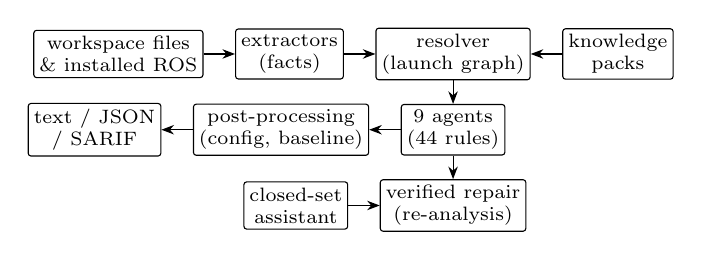
\begin{tikzpicture}[node distance=3mm and 4mm, every node/.style={font=\scriptsize},
  box/.style={draw, rounded corners=1pt, align=center, minimum height=6mm, inner sep=2pt},
  >={Stealth[length=1.6mm]}]
\node[box] (files) {workspace files\\ \& installed ROS};
\node[box, right=of files] (ext) {extractors\\(facts)};
\node[box, right=of ext] (res) {resolver\\(launch graph)};
\node[box, below=of res] (ag) {9 agents\\(44 rules)};
\node[box, left=of ag] (pp) {post-processing\\(config, baseline)};
\node[box, left=of pp] (out) {text / JSON\\ / SARIF};
\node[box, below=of ag] (fix) {verified repair\\(re-analysis)};
\node[box, left=of fix] (assist) {closed-set\\assistant};
\node[box, right=of res] (pack) {knowledge\\packs};
\draw[->] (files) -- (ext);
\draw[->] (ext) -- (res);
\draw[->] (pack) -- (res);
\draw[->] (res) -- (ag);
\draw[->] (ag) -- (pp);
\draw[->] (pp) -- (out);
\draw[->] (ag) -- (fix);
\draw[->] (assist) -- (fix);
\end{tikzpicture}
\caption{Architecture of \tool.}
\label{fig:arch}
\end{figure}

\subsection{Fact extraction}

Extractors exist for \code{package.xml}; a small CMake interpreter (variables, executables,
libraries, \code{install} rules, ament\_cmake\_auto, rclcpp component registration,
generate\_parameter\_library specs); \code{setup.py}/\code{setup.cfg}; launch files in XML,
YAML and Python; parameter YAML; C++ (via tree-sitter~\cite{treesitter}); Python (via the
RustPython AST); URDF with a xacro subset (properties, arguments, arithmetic, macros with block
parameters, includes, conditionals); SROS2 governance, permissions and policy documents; and
RViz configurations, whose displays carry their own QoS.

Python launch files are \emph{not executed}. A static interpreter evaluates the common
subset---\code{Node}, \code{IncludeLaunchDescription}, \code{GroupAction},
\code{PushRosNamespace}, \code{SetParameter}, \code{DeclareLaunchArgument},
\code{LaunchConfiguration}, path substitutions, helper functions defined in the file, and
Nav2's \code{RewrittenYaml}/\code{ParameterFile}---and marks anything else as unknown.

The parameter-YAML layer keeps exact byte spans and types scalars like
\code{rcl\_yaml\_param\_parser} (e.g.\ \code{on} is a boolean, \code{1} an integer, \code{1.0}
a double, quoted values strings), so that type checks reflect runtime behaviour and every finding
points at the exact key or value.

From C++ and Python nodes the extractors record the node name, declared parameters with types
and defaults, publishers, subscriptions, clients and services with literal names and QoS,
callbacks (lambdas, \code{std::bind} member functions, Python methods), callback groups,
executors, and blocking calls. QoS expressions are evaluated statically, including presets,
chained modifiers and statement-level modifications of local QoS variables; project-specific
QoS classes whose policy cannot be determined are recorded as unknown.

\subsection{Resolved launch graph}
\label{sec:graph}

Every launch file is a root. The resolver walks its items, follows includes into workspace and
installed packages, and propagates launch arguments (a value passed by the includer overrides
the included file's default). Namespaces follow ROS~2 rules: relative pushes compose, absolute
ones reset. Scoped groups restore namespace, parameters and remappings.

For each node it computes the fully qualified name, binds parameters from inline values,
\code{SetParameter} and parameter files, and applies remappings by comparing fully expanded
names. Parameter-file sections are matched like \code{rcl}: a key $k$ applies to node $n$ iff
\begin{equation}
\mathrm{match}\big(\mathrm{abs}(k), \mathrm{fqn}(n)\big),\quad
\mathrm{abs}(k) = \begin{cases} k & k \text{ starts with } / \\ /k & \text{otherwise}\end{cases}
\end{equation}
where \code{*} matches one name token and \code{**} any number of tokens. For
\code{RewrittenYaml(root\_key=$r$)} keys are prefixed with $r$.

Each launched node is linked to its implementation: the executable is looked up in the
package's build rules, its source files (including sources of linked in-package libraries) are
collected, and node classes defined there---and the same classes in other files of the package,
such as headers---become its implementation. Composable nodes are linked through their plugin
class.

\subsection{Precision first}
\label{sec:precision}

A static checker for configuration loses users quickly through false positives, so every fact
carries what could not be determined, and every rule checks those markers before reporting.
The most important case is parameter declarations. We distinguish three levels:
\emph{closed} (all declarations known), \emph{dotted-open} (declarations of names containing
a dot are uncertain, e.g.\ because the node loads plugins whose parameters are
\code{plugin\_name.param}), and \emph{open} (a declaration with a fully dynamic name). P003
reports an undeclared parameter only if the node is closed, or if it is dotted-open and the
parameter name contains no dot.

Declarations made through another object's node handle (parameter-handler classes, plugin
interfaces, header-only library helpers) are attributed to a node class when possible; literal
declarations found in the node's workspace dependency closure are accepted; and a node whose
base class is not a standard ROS node class and cannot be found in that closure is treated as
open. A text fallback recovers declarations that the C++ grammar cannot parse without type
information (e.g.\ \code{declare\_or\_get\_parameter<T>("x")}, which parses as a comparison);
it is only used to \emph{accept} names, never to report them.

Similar markers exist elsewhere: a launch graph containing unresolved includes or dynamic code
is \emph{partial}; topic checks that need a closed world are only reported when every node in
the graph was linked to source; robot models containing unexpanded xacro are lenient.

\subsection{Installed environment and knowledge packs}
\label{sec:installed}

Real launch files start packages the developer did not write. In a sourced ROS shell \tool{}
reads the ament resource index~\cite{ament_index} of every prefix in \code{AMENT\_PREFIX\_PATH}:
installed packages, their executables (\code{lib/<pkg>}), pluginlib plugins (resource types
\code{<category>\_\_pluginlib\_\_plugin}), rclcpp components and dependencies. Launch and
parameter files of installed packages that the workspace includes are loaded so that includes
resolve; findings are never reported inside them. Plugin catalogs used for typo detection come
from the installed index rather than from hand-written lists.

Binary installs contain no source code, so the parameters an installed node declares are
unknown. A \emph{knowledge pack} provides them: \tool's own extractors and linker are run once
over the source of popular packages at each distribution's branch, and the resulting per-node
facts (parameters with types and defaults, openness level, endpoints with QoS) are embedded in
the binary. Table~\ref{tab:packs} summarises the packs built from nine upstream repositories
(Nav2, ros2\_controllers, ros2\_control, robot\_state\_publisher, joint\_state\_publisher,
geometry2, demos, slam\_toolbox, robot\_localization). Packs are used only when the
distribution is known, because parameter names change between distributions.

\begin{table}[t]
\centering
\caption{Embedded knowledge packs}
\label{tab:packs}
\footnotesize
\begin{tabular}{@{}lrrrrr@{}}
\toprule
Distribution & Packages & Executables & Components & Parameters & Size \\
\midrule
Humble & 40 & 100 & 52 & 2{,}596 & 11\,KiB\\
Jazzy  & 44 &  96 & 38 & 3{,}850 & 14\,KiB\\
Kilted & 44 &  97 & 37 & 3{,}711 & 14\,KiB\\
\bottomrule
\end{tabular}
\end{table}

\subsection{Verified repair}
\label{sec:repair}

Agents attach a fix to a finding only when the edit is local and mechanical (e.g.\
\code{1}$\to$\code{1.0}, renaming a misspelled key to the closest declared name, adding a
\code{<depend>}, installing \code{launch/}). Algorithm~\ref{alg:fix} shows how fixes are
accepted: they are applied in memory, the whole workspace is re-analysed, and a fix is kept only
if its finding disappears and no new error appears in the touched files. Accepted fixes are
written atomically (temporary file and rename); without \code{--write} they are only shown as a
diff.

\begin{algorithm}[t]
\caption{Fix verification}
\label{alg:fix}
\footnotesize
\begin{algorithmic}[1]
\State $F \gets$ non-overlapping fixes of all findings $D$
\For{round $=1..3$}
  \State $W' \gets$ workspace with $F$ applied in memory
  \State $D' \gets \mathrm{analyse}(W')$
  \State $R \gets \{f\in F \mid \mathrm{finding}(f)\in D' \lor \mathrm{newErrors}(D', D, f)\}$
  \If{$R=\emptyset$} \Return $F$ \EndIf
  \State $F \gets F \setminus R$
\EndFor
\State \Return $F$
\end{algorithmic}
\end{algorithm}

\paragraph{Closed-set repair assistant}
Some findings have no mechanical fix, e.g.\ a key \code{max\_lin\_vel} for a node that declares
\code{max\_linear\_velocity}, \code{min\_linear\_velocity} and \code{controller\_frequency}: the
edit distance is too large for typo correction. Such findings carry a \emph{repair site}: the
exact span and the closed set of values that are valid there (declared parameters, joints in
\code{<ros2\_control>}, URDF frames, installed executables, known enclaves). The assistant only
chooses one of these values or abstains; it never generates text. A lexical ranker combines edit
distance, word overlap and expansion of common ROS abbreviations (\code{vel}, \code{freq},
\code{ctrl}, \dots). A learned ranker---a 16$\to$16$\to$1 multilayer perceptron over 16 string
features (edit distances, character $n$-gram overlap, prefix and subsequence coverage, rank
features), about 290 weights compiled into the binary---scores the candidates of one finding
jointly through a softmax. A choice is accepted only with a clear margin over the runner-up, is
then verified by Algorithm~\ref{alg:fix}, and is labelled \emph{assisted}. Because
re-analysis proves that a finding disappears but not that the chosen value is the intended one,
assisted fixes are written only with an explicit flag.

We first prototyped the assistant with a 0.5B-parameter code language model (the
off-the-shelf base model, 4-bit quantised) answering a multiple-choice prompt, run on the CPU
with a pure-Rust inference library. Loading took 4.5\,s and scoring a 151-token prompt took
17.6\,s on a laptop CPU in a portable x86-64 build without AVX2 kernels. For a
closed-set choice between string candidates the small ranker is several orders of magnitude
cheaper, needs no model files and keeps the tool's footprint unchanged; we therefore adopted it.

\paragraph{Sandboxed build check}
With \code{--verify-build}, the workspace is copied twice to a temporary directory, the fixes are
applied to one copy, and both are built with \code{colcon}---inside a ROS container with
networking disabled when Docker is available. Fixes are refused if the original builds and the
patched copy does not; if the original does not build, the check is inconclusive. The user's
tree is never built.

\paragraph{Optional references}
With \code{--online}, findings receive links to related Robotics Stack Exchange questions and
GitHub issues of the ROS organisations. Queries are built only from the rule that fired
(e.g.\ ``ros2 parameter not declared yaml value ignored''), so no file content, path or name
leaves the machine. A separate helper process performs the requests against an allowlist of
HTTPS hosts with no redirects, a 5\,s timeout and a 256\,KiB response limit; results are cached
and are shown to the user only, never used for edits.

\subsection{Implementation and distribution}

\tool{} is written in Rust (about 15{,}000 lines). It runs single-threaded by default (an
opt-in feature parallelises file extraction), reports text, versioned JSON and
SARIF~2.1.0~\cite{sarif} with rule metadata, exact regions and fixes, supports inline
suppressions and baselines for gradual adoption, and returns a non-zero exit code when findings
reach a configurable severity. Packaging is provided for Python wheels containing the binary
(also providing a \code{ros2 rosfix} command), standalone archives, container images with a ROS
distribution, a GitHub Action and pre-commit hooks.

% ===========================================================================
\section{Evaluation}
\label{sec:eval}

We ask: \textbf{RQ1} How precise is \tool{} on real code? \textbf{RQ2} Does it detect injected
misconfigurations at the right location? \textbf{RQ3} How much of a large system does the
analysis cover? \textbf{RQ4} What does it cost?

\paragraph{Setup}
We analysed shallow clones of five public repositories (Table~\ref{tab:real}) with a release
build on a Windows laptop (12 logical CPUs, 16\,GB RAM), single-threaded, with a cold file cache
and without a ROS installation. Packs were not used in RQ1--RQ4 because no distribution was set.

\subsection{RQ1: Precision on real code}

Table~\ref{tab:real} lists all findings; we reviewed every one manually.
The L002 findings are missing \code{package.xml} dependencies, e.g.\
\code{turtlebot3\_bringup} starts nodes from \code{rclcpp\_components}, \code{camera\_ros}
and \code{image\_view} without declaring them, and example launch files of
\code{nav2\_simple\_commander} start \code{ros\_gz\_sim} and \code{robot\_state\_publisher}
without declaring them. These do not fail in a developer's workspace but break installation from
binaries. E002 findings are sleeps inside action-server and subscription callbacks executed by
the executor (in tutorials and demos). S002 findings are example nodes of Nav2 started next to
a simulator without \code{use\_sim\_time}; they are correct but low-impact. We found no false
positives among the reported findings.

For comparison, the previous rule set of the same project reported 617 findings on these
repositories; 305 were calls to \code{spin\_until\_future\_complete}, 254 of them (83\%) in test
code where this call is the intended API, and a manual check of 35 sampled findings found no real
defect.

\begin{table}[t]
\centering
\caption{Analysis of five public repositories (cold cache, one thread)}
\label{tab:real}
\footnotesize
\begin{tabular}{@{}lrrrl@{}}
\toprule
Repository & Files & Time & Memory & Findings\\
\midrule
ros2/demos                 & 138 & 1.3\,s &  13\,MB & E002$\times$2, L002$\times$6\\
ros2/sros2                 &  20 & 0.1\,s &   5\,MB & ---\\
turtlebot3                 &  63 & 0.1\,s &  12\,MB & E002$\times$2, L002$\times$5\\
ros2\_control              & 124 & 0.7\,s &  20\,MB & ---\\
navigation2                & 732 & 5.1\,s &  68\,MB & L002$\times$31, S002$\times$10\\
\bottomrule
\end{tabular}
\end{table}

\paragraph{False-positive sources found on real code}
Analysing Nav2 and the other repositories during development exposed false positives that unit
tests had not, each caused by an incomplete model of ROS~2 practice: parameter files passed
through \code{ParameterFile(RewrittenYaml(\dots))}; nested dictionaries in Python launch
parameters, which ROS flattens to dotted names; project-specific QoS classes such as
\code{LatchedPublisherQoS}; launch\_testing files without \code{generate\_launch\_description};
callbacks that hand work to a thread; dependencies declared through metapackages; the member
form of \code{declare\_or\_get\_parameter}; parameters declared by shared library code in
dependency packages; and template calls misparsed without type information. Each was fixed in
the extractors or the resolver rather than by suppressing rules.

\subsection{RQ2: Detection of injected misconfigurations}

A mutation benchmark injects one realistic fault at a time, \emph{in memory}, at a site found
in the clean analysis---for example, a parameter that a node really declares and that a launch
file really binds. A mutation counts as detected only if the expected rule fires at the mutated
line (for removed dependencies: a finding naming the dependency and package). Dependencies that
remain available through another declared package are not removed, since \tool{} deliberately
accepts metapackage dependencies. Table~\ref{tab:mut} shows the results: all 107 mutations were
detected. In addition, three faults injected by hand into Nav2's default parameter file (a
misspelled \code{controller\_frequency}, an integer for a double, and a misspelled
\code{ros\_\_parameters}) were detected, each with a correct verified fix.

\begin{table}[t]
\centering
\caption{Mutation benchmark on the five repositories}
\label{tab:mut}
\footnotesize
\begin{tabular}{@{}llrr@{}}
\toprule
Mutation & Rule & Injected & Detected\\
\midrule
parameter key typo                   & P003 & 10 & 10\\
double written as integer            & P004 &  7 &  7\\
\code{ros\_\_parameters} misspelled  & P002 & 33 & 33\\
executable name typo in launch file  & L001 & 21 & 21\\
dependency removed from package.xml  & L002 & 16 & 16\\
Nav2 plugin type typo                & N002 & 20 & 20\\
\midrule
total                                &      & 107 & 107\\
\bottomrule
\end{tabular}
\end{table}

These mutations are synthetic single faults whose operators were written alongside the tool. The
result shows that the checks work on real code layouts; it is not an estimate of recall on
faults developers actually make.

\paragraph{Installed packages}
With the Jazzy pack, a workspace that launches Nav2's installed controller server with
\code{controller\_frequency: 20} is reported as a type error that crashes the node at startup,
with the fix \code{20.0}, and a misspelled \code{min\_x\_velocity\_treshold} as undeclared---without
Nav2's source on the machine. Without a distribution, only the catalog-based typo rule N006 fires.

\subsection{RQ3: Coverage}

In navigation2, \tool{} built 50 launch graphs with 1{,}161 node instances; 1{,}065 were linked to
source code. Parameter checking applies fully to 132 of them, to all top-level names for 877
plugin-hosting nodes (dotted-open), and is disabled for 56 nodes whose declarations cannot be
determined. Before the openness levels and declaration attribution of
Sec.~\ref{sec:precision} were introduced, 1{,}048 of the linked nodes were fully open.

\subsection{RQ4: Cost}

Table~\ref{tab:real} reports wall time and peak memory: at most 5.1\,s and 68\,MB for
navigation2 with a cold cache (warm runs are several times faster). Online references for the
example of Sec.~\ref{sec:repair} required one query and 1.2\,s, and none on the next run (cache).

% ===========================================================================
\section{Related Work}

\paragraph{Static analysis of ROS systems}
HAROS~\cite{santos2016haros,santos2021haros} pioneered quality analysis and model extraction for
ROS repositories. ROSDiscover~\cite{timperley2022rosdiscover} statically recovers the run-time
architecture of ROS~1 systems from code and launch files and checks it against rules;
ROSInfer~\cite{durschmid2024rosinfer} infers behavioural component models. QoS
Guard~\cite{lee2025qosguard} formalises dependency rules between DDS QoS policies and checks
XML profiles offline. LiSA4ROS2~\cite{zanatta2024lisa} uses abstract interpretation of Python
nodes to derive SROS2 access policies. phriky-units~\cite{ore2017phriky} detects physical
unit inconsistencies in C++. \tool{} differs by resolving a ROS~2 launch graph across launch
files, parameter files, code, packaging and installed packages, and by verifying its repairs.

\paragraph{Empirical studies and datasets}
Canelas et al.~\cite{canelas2024misconfig} catalogue ROS misconfigurations and the techniques
that address them; Chen et al.~\cite{chen2025ibugs} study interaction bugs; ROBUST provides 221
reproducible ROS bugs~\cite{timperley2024robust}. These motivate our rule selection.

\paragraph{Dynamic analysis and security}
ros2\_tracing~\cite{bedard2022tracing} and response-time analysis of
executors~\cite{casini2019rta} address timing; fuzzers such as RoboFuzz~\cite{kim2022robofuzz}
find correctness bugs at runtime. Security tooling and analyses of SROS2 are described
in~\cite{mayoral2022sros2,deng2022secureros2}. These are complementary to static checking.

\paragraph{Program repair}
Learning-based repair commonly fine-tunes code models~\cite{silva2023repairllama} and benefits
from retrieved fix examples~\cite{wang2023rapgen}. Our setting is narrower: the valid repairs
are enumerable from the analysis, so the assistant ranks a closed set instead of generating
code, and every choice is verified.

% ===========================================================================
\section{Limitations and Threats to Validity}

\emph{Static scope.} Values computed at runtime, names built from runtime data and code executed
by \code{OpaqueFunction} are not analysed; such parts are marked partial and checks are
suppressed. The xacro and Python-launch interpreters cover common subsets only.
\emph{External validity.} Five repositories and one machine do not represent all ROS~2
projects; the mutation operators are synthetic and were written by the authors of the tool.
\emph{Manual review.} Findings were reviewed by one author.
\emph{Packs.} Knowledge packs reflect the branches they were built from and can lag behind
installed versions; they are disabled when the distribution is unknown.
\emph{Assistant.} The learned ranker's weights must be trained on mutation and mined data; at
the time of writing the shipped weights reproduce the lexical ranker, and we report no accuracy
for the learned model. The sandboxed build check was not exercised in the evaluation, which ran
without Docker or a ROS installation.

% ===========================================================================
\section{Conclusion and Future Work}

\tool{} shows that a large class of silent ROS~2 misconfigurations can be detected statically
once the launch graph is resolved with the semantics of the launch system and \code{rcl}, and
that precision on real code depends on modelling ROS practice---rewritten parameter files,
plugin-declared parameters, metapackages---rather than on rule-specific heuristics. Future work
is a benchmark of real historical misconfiguration fixes mined from permissively licensed ROS~2
repositories and verified by the tool, training and evaluating the learned ranker on it,
analysing runtime-generated launch descriptions, and studying adoption in continuous
integration.

\section*{Availability}
\tool, the knowledge-pack builder, the mutation benchmark and the evaluation scripts are
available at \url{https://github.com/SohamWalam11/ros2-safety-lint}.

\bibliographystyle{IEEEtran}
\bibliography{references_rewrite}

\end{document}
